\documentclass{beamer}
\usepackage{hyperref}
\usepackage{csquotes}
\usepackage{graphicx}

\title{GitHub}
\author{Edwin Kofler}
\hypersetup{
	colorlinks=true
}
\pdfinfo{
	/keywords (Git;GitHub)
}
\graphicspath{ {./assets} }


\begin{document}
\frame{\titlepage}

\begin{frame}{Agenda}
	\begin{enumerate}
		\item About Me
		\item Introduce Git
		\item Introduce GitHub
		\item Tour of GitHub
		\item Resources
	\end{enumerate}
\end{frame}

\begin{frame}
	\begin{columns}
		\begin{column}{0.48\textwidth}
			
\includegraphics{panda-500px.jpg} \newline
			{ \tiny Image by Art G. on \href{https://www.flickr.com/photos/digitalart/4084550022}{Flickr}; licensed as CC BY-NC-ND 2.0 }
		\end{column}
		\begin{column}{0.48\textwidth}
			{\Huge Edwin Kofler} \newline
			\begin{itemize}
				\item \href{https://edwinkofler.com/}{Website}
				\item \href{https://github.com/hyperupcall}{GitHub}
				\item \href{https://twitter.com/hyperupcall}{Twitter}
				\item \href{https://www.linkedin.com/in/hyperupcall}{LinkedIn}
			\end{itemize}
		\end{column}
	\end{columns}
\end{frame}

\begin{frame}{Introducing Git}
	From the official Git \href{https://git-scm.com}{website}: \newline

	\begin{displayquote}
		Git is a \href{https://git-scm.com/about/free-and-open-source}{free and open source} distributed version control system...
	\end{displayquote}

	{
	\small

	But what does that mean in practice? Git...

	\begin{itemize}
		\item Lets you ``look at" a file at a previous point in time
		\item Allows multiple people to work on the same codebase at a time
		\item Lets you experiment with your code (and keep the original copy safe)
	\end{itemize}
	}

	\href{https://raw.githubusercontent.com/ecc-cs-club/slides/main/1-Git-And-GitHub/assets/using-git.png}{
		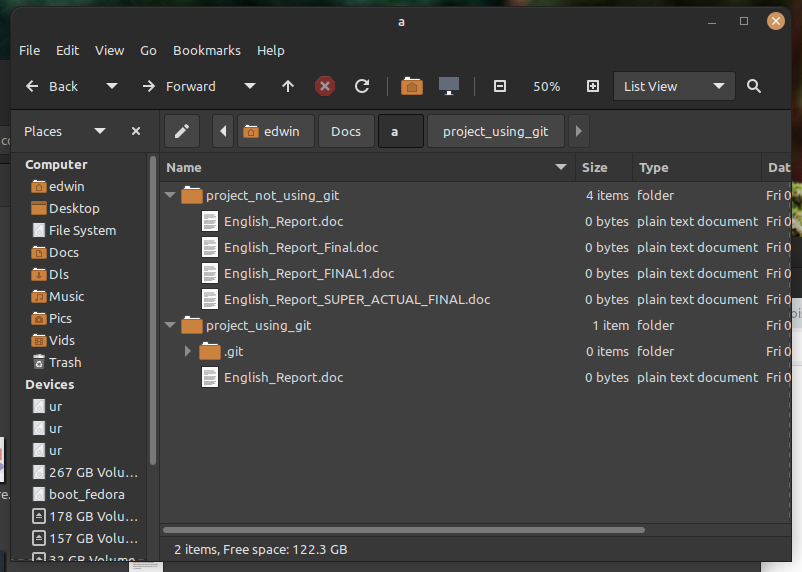
\includegraphics[width=6cm]{using-git.png}
	}


	\note{
		multiple people to work - if no git, would have to work on same computer. sometimes have trouble opening up files
		history - from a ``single file" to many many files like in those big projects
	}
\end{frame}

\begin{frame}{Introducing GitHub}
	\begin{itemize}
		\item Sort of a combination of Dropbox and Twitter
		\item Better to show, than tell...
	\end{itemize}

	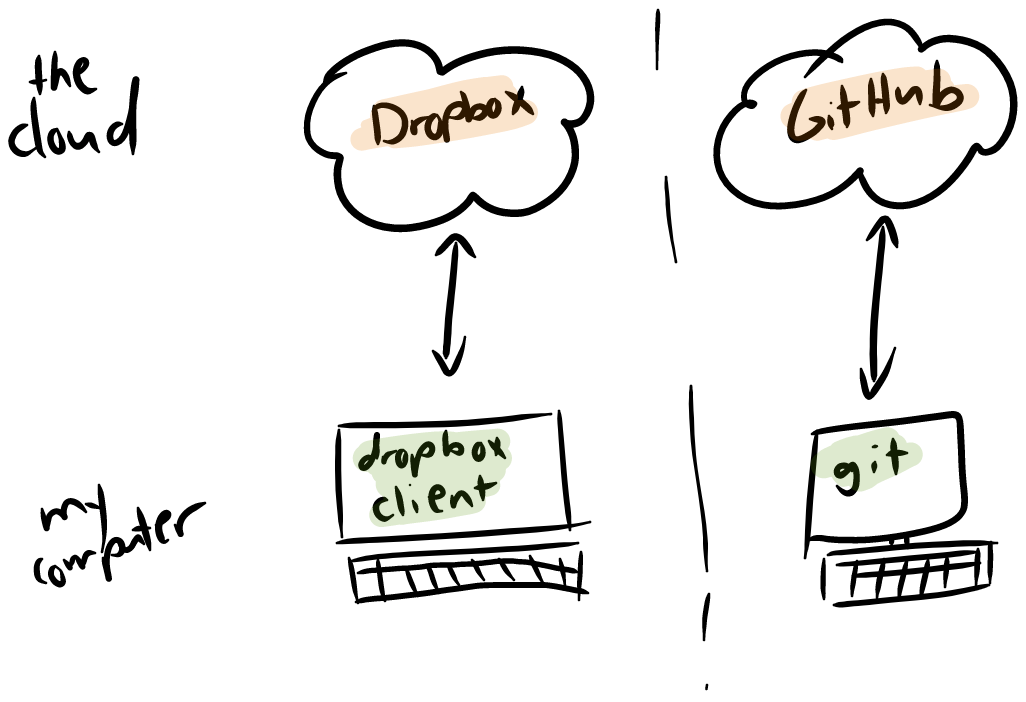
\includegraphics[width=10cm]{dropbox-github.png} \newline

	\note{
		Like Dropbox, sort of ``syncing" a folder on your computer with a remote server

		There is a \href{https://docs.github.com/en/get-started/signing-up-for-github/signing-up-for-a-new-github-account}{help page}, but it does not offer useful information
	}
\end{frame}

\begin{frame}{Tour of GitHub}
	\begin{itemize}
		\item Create GitHub account
		\item Explore ``home" view
		\item Show ``profile" view
		\item Create a ``profile README"
		\item Show small repository: \href{https://github.com/fox-projects/xdgbasedirectoryspecification.com}{fox-projects/xdgbasedirectoryspecification.com}
		\item Show large repository: \href{https://github.com/xournalpp/xournalpp}{xournalpp/xournalpp}
	\end{itemize}

	\note{
		- in issues: ``good first issue"
		- show pull requests
	}
\end{frame}

\end{document}
